% Options for packages loaded elsewhere
\PassOptionsToPackage{unicode}{hyperref}
\PassOptionsToPackage{hyphens}{url}
\PassOptionsToPackage{dvipsnames,svgnames,x11names}{xcolor}
%
\documentclass[
  12pt,
]{article}
\title{~\Large Eras in baseball: Change point analysis fun title.}
\author{\large Mena Whalen \vspace{-1.1mm}\\
\normalsize Department of Mathematics and Statistics \vspace{-1mm}\\
\normalsize Loyola University Chicago \vspace{-1mm}\\
\normalsize Chicago, IL 60660 \vspace{-1mm}\\
\normalsize \href{mailto:mwhalen3@luc.edu}{\texttt{mwhalen3@luc.edu}}
\vspace{-1mm}\\
\strut \\
\large Gregory J. Matthews \vspace{-1.1mm}\\
\normalsize Department of Mathematics and Statistics \vspace{-1mm}\\
\normalsize Loyola University Chicago \vspace{-1mm}\\
\normalsize Chicago, IL 60660 \vspace{-1mm}\\
\normalsize \href{mailto:gmatthews1@luc.edu}{\texttt{gmatthews1@luc.edu}}
\vspace{-1mm}}
\date{}

\usepackage{amsmath,amssymb}
\usepackage{lmodern}
\usepackage{iftex}
\ifPDFTeX
  \usepackage[T1]{fontenc}
  \usepackage[utf8]{inputenc}
  \usepackage{textcomp} % provide euro and other symbols
\else % if luatex or xetex
  \usepackage{unicode-math}
  \defaultfontfeatures{Scale=MatchLowercase}
  \defaultfontfeatures[\rmfamily]{Ligatures=TeX,Scale=1}
\fi
% Use upquote if available, for straight quotes in verbatim environments
\IfFileExists{upquote.sty}{\usepackage{upquote}}{}
\IfFileExists{microtype.sty}{% use microtype if available
  \usepackage[]{microtype}
  \UseMicrotypeSet[protrusion]{basicmath} % disable protrusion for tt fonts
}{}
\makeatletter
\@ifundefined{KOMAClassName}{% if non-KOMA class
  \IfFileExists{parskip.sty}{%
    \usepackage{parskip}
  }{% else
    \setlength{\parindent}{0pt}
    \setlength{\parskip}{6pt plus 2pt minus 1pt}}
}{% if KOMA class
  \KOMAoptions{parskip=half}}
\makeatother
\usepackage{xcolor}
\IfFileExists{xurl.sty}{\usepackage{xurl}}{} % add URL line breaks if available
\IfFileExists{bookmark.sty}{\usepackage{bookmark}}{\usepackage{hyperref}}
\hypersetup{
  colorlinks=true,
  linkcolor={cyan},
  filecolor={Maroon},
  citecolor={Blue},
  urlcolor={cyan},
  pdfcreator={LaTeX via pandoc}}
\urlstyle{same} % disable monospaced font for URLs
\usepackage[margin=1in]{geometry}
\usepackage{longtable,booktabs,array}
\usepackage{calc} % for calculating minipage widths
% Correct order of tables after \paragraph or \subparagraph
\usepackage{etoolbox}
\makeatletter
\patchcmd\longtable{\par}{\if@noskipsec\mbox{}\fi\par}{}{}
\makeatother
% Allow footnotes in longtable head/foot
\IfFileExists{footnotehyper.sty}{\usepackage{footnotehyper}}{\usepackage{footnote}}
\makesavenoteenv{longtable}
\usepackage{graphicx}
\makeatletter
\def\maxwidth{\ifdim\Gin@nat@width>\linewidth\linewidth\else\Gin@nat@width\fi}
\def\maxheight{\ifdim\Gin@nat@height>\textheight\textheight\else\Gin@nat@height\fi}
\makeatother
% Scale images if necessary, so that they will not overflow the page
% margins by default, and it is still possible to overwrite the defaults
% using explicit options in \includegraphics[width, height, ...]{}
\setkeys{Gin}{width=\maxwidth,height=\maxheight,keepaspectratio}
% Set default figure placement to htbp
\makeatletter
\def\fps@figure{htbp}
\makeatother
\setlength{\emergencystretch}{3em} % prevent overfull lines
\providecommand{\tightlist}{%
  \setlength{\itemsep}{0pt}\setlength{\parskip}{0pt}}
\setcounter{secnumdepth}{5}
\newlength{\cslhangindent}
\setlength{\cslhangindent}{1.5em}
\newlength{\csllabelwidth}
\setlength{\csllabelwidth}{3em}
\newlength{\cslentryspacingunit} % times entry-spacing
\setlength{\cslentryspacingunit}{\parskip}
\newenvironment{CSLReferences}[2] % #1 hanging-ident, #2 entry spacing
 {% don't indent paragraphs
  \setlength{\parindent}{0pt}
  % turn on hanging indent if param 1 is 1
  \ifodd #1
  \let\oldpar\par
  \def\par{\hangindent=\cslhangindent\oldpar}
  \fi
  % set entry spacing
  \setlength{\parskip}{#2\cslentryspacingunit}
 }%
 {}
\usepackage{calc}
\newcommand{\CSLBlock}[1]{#1\hfill\break}
\newcommand{\CSLLeftMargin}[1]{\parbox[t]{\csllabelwidth}{#1}}
\newcommand{\CSLRightInline}[1]{\parbox[t]{\linewidth - \csllabelwidth}{#1}\break}
\newcommand{\CSLIndent}[1]{\hspace{\cslhangindent}#1}
\usepackage{setspace} \setstretch{1.15} \usepackage{float} \floatplacement{figure}{t}
\ifLuaTeX
  \usepackage{selnolig}  % disable illegal ligatures
\fi

\begin{document}
\maketitle
\begin{abstract}
Baseball is some weird and wild shit. \vspace{2mm}\\
\emph{Keywords}: change point analysis, baseball,
\end{abstract}

\newpage

\hypertarget{sec:intro}{%
\section{Introduction}\label{sec:intro}}

The first professional baseball team in the United States, the
Cinicnnati Red Stockings, was formed in 1869
(\protect\hyperlink{ref-BBHOF1869}{Rothenberg}
(\protect\hyperlink{ref-BBHOF1869}{n.d.})). Many leagues came and went
in the late 1800s, but National League (NL), formed in 1876, emerged as
the predominant league of the time. A few decades later, the American
League (AL) began growing in popularity and eventually reached an
agreement with the NL to be the two major leagues of baseball with the
winner of each league playing in the World Series starting in 1903.

Throughout the history of baseball in the United States, the game has
gone through many changes and distinct eras. For example, the time
period between approximately 1900-1919 is often referred to as the
``Dead Ball Era'' and was marked by low scoring games and dominant
pitching. Another more recent example would be the ``Steroid Era'' which
lasted from approximately 1994 through 2005 and was characterized by a
rapid increase in power hitting largely attributed to players using
performance enhancing drugs.

While many baseball writers have attempted to define the different eras
of baseball, there has also been some academic work that has sought to
empirically define eras in baseball.
\protect\hyperlink{ref-Groothius2017}{Groothius, Rotthoff, and
Strazicich} (\protect\hyperlink{ref-Groothius2017}{2017}) looked for
structural breaks in univariate times series of performance measures
over the period from 1871-2020. They analyzed four statistics: slugging
percentage (SLG, home run (HR) rate, batting average (BA), and runs
batted in (RBI) rate. For each of these statistics, the computed the
mean and standard deviation (SD) across all players who had at least 100
at bats in a given season to yield a univariate time series for each of
these statistics. They then used the Lagrange Multiplier (LM) unit root
test proposed in
(\protect\hyperlink{ref-LeeandStrazicich2003}{\textbf{LeeandStrazicich2003?}})
to find structural breaks. They identified structural breaks in slugging
percentage in 1921 and 1992, the first of which marks the end of the
Dead Ball Era and the latter corresponding to the start of the steroid
era.

\protect\hyperlink{ref-LeeFort2005}{H. and R.}
(\protect\hyperlink{ref-LeeFort2005}{2005}) looks for structural changes
in competitive balance of the two league American and National. Use
methods from Andrews1993, Bai1997, 1999 and Bai and Perron 1998 and 2003
to look for break points between 1901 -1999. Theuy measure competitive
balance in two ways: 1) Noll 1988 and Scully 1989 and 2) Lee (2004).
They find break point sin competitive balance in 1912, 1926, and 1933
for the NL and in 1926 and 1957 in the AL.

Baseball is not the only sport where this type of analysis has been
applied. \protect\hyperlink{ref-PalaciosHuerta2004}{I.}
(\protect\hyperlink{ref-PalaciosHuerta2004}{2004}) looked for structural
changes in soccer using data from British soccer leagues through 1996.
\protect\hyperlink{ref-FortLee2007}{Fort R.}
(\protect\hyperlink{ref-FortLee2007}{2007}) looked for structural breaks
in major North American sports other than baseballl; that is basketball
(NBA), hockey (NHL), and American football (NFL). WHAT DID THEY FIND?

All of the previous work mentioned here focuses on
\textbf{\emph{univariate}} In contrast to their methods, we use more
modern methods Double CUSUM Binary Segmentation algorithm
(\protect\hyperlink{ref-Cho2016}{H. Cho}
(\protect\hyperlink{ref-Cho2016}{2016})) and the Sparsified Binary
Segmentation algorithm (\protect\hyperlink{ref-ChoFryzlewwicz2014}{H.
Cho and Fryzlewicz} (\protect\hyperlink{ref-ChoFryzlewwicz2014}{2014})).

Just Notes: Palacios-Huerta I. (2004). Structural changes during a
Century of the World's most popular sport. Statistical Methods and
Applications, 13, 241--258
\protect\hyperlink{ref-PalaciosHuerta2004}{I.}
(\protect\hyperlink{ref-PalaciosHuerta2004}{2004}) Structural Breaks in
soccer

\protect\hyperlink{ref-Nieswiadomy2012}{Nieswiadomy}
(\protect\hyperlink{ref-Nieswiadomy2012}{2012}) Was there a structural
break in Barry Bonds's Bat? Looking for structural breaks in Bonds OPS
times series. Use the uni root test on monthly data from 86-07. The
identify break points in June 1993 and Sept 2000.

In contrast to their methods, we use more modern methods Double CUSUM
Binary Segmentation algorithm (\protect\hyperlink{ref-Cho2016}{H. Cho}
(\protect\hyperlink{ref-Cho2016}{2016})) and the Sparsified Binary
Segmentation algorithm (\protect\hyperlink{ref-ChoFryzlewwicz2014}{H.
Cho and Fryzlewicz} (\protect\hyperlink{ref-ChoFryzlewwicz2014}{2014})).

\url{https://onlinelibrary.wiley.com/doi/epdf/10.1111/j.1465-7295.2007.00026.x}
Fort and Lee 2007: Looks for structural breaks in NBA, NHL, and NFL

\url{https://www.baseball-reference.com/bullpen/History_of_baseball_in_the_United_States}

\url{https://thesportjournal.org/article/examining-perceptions-of-baseballs-eras/}

SOME MORE STUFF

\url{https://pubmed.ncbi.nlm.nih.gov/30747582/}?

The goal of this work is to use multivariate change point analysis to
identify change points in MLB as a whole to objectively identify eras in
the games history, but also to look for change points to identify team
specific eras.

The work that is the most closely related to our own is that of
\protect\hyperlink{ref-Groothius2017}{Groothius, Rotthoff, and
Strazicich} (\protect\hyperlink{ref-Groothius2017}{2017}), which looked
for structural breaks (Note: the terms ``structural breaks'' and
``change points'' are used interchangeably in this manuscript) in
univariate times series.

univariate time series of the means and SD's of several statistics
(i.e.~SLUG, HR rate, RBI rate, and batting average) to look for
structural breaks via the Lagrange Multiplier (LM) unit root test
(\protect\hyperlink{ref-LeeandStrazicich2003}{\textbf{LeeandStrazicich2003?}}).
Notably they find structural breaks in slugging percentage in 1921 and
1992. In contrast to their methods, we use more modern methods Double
CUSUM Binary Segmentation algorithm (\protect\hyperlink{ref-Cho2016}{H.
Cho} (\protect\hyperlink{ref-Cho2016}{2016})) and the Sparsified Binary
Segmentation algorithm (\protect\hyperlink{ref-ChoFryzlewwicz2014}{H.
Cho and Fryzlewicz} (\protect\hyperlink{ref-ChoFryzlewwicz2014}{2014})).

\protect\hyperlink{ref-Woltring2018}{Woltring and Jubenville}
(\protect\hyperlink{ref-Woltring2018}{2018}) From Woltring: ``Baseball
has endured much change over the course of its history, and because of
constant change, the modern era of baseball has been segmented into six
distinct sub-eras. A common list presented at Baseball-Reference
described the eras as the Dead Ball Era (1901-1919), the Live Ball Era
(1920-1941), the Integration Era (1942-1960), the Expansion Era
(1961-1976), the Free Agency Era (1977-1993) and the Long Ball/Steroid
Era (1994-2005) (17). This study runs through the 2011 season and a
seventh era will be added and labeled the Post Steroid Era (2006-2011)''

Deadball era:
\url{https://sabr.org/journal/article/the-rise-and-fall-of-the-deadball-era/}

\url{http://mlb.mlb.com/mlb/history/mlb_history_people.jsp?story=com}

\url{https://www.nytimes.com/2011/09/25/sports/baseball/scoring-in-baseball-returns-to-dead-ball-levels.html?_r=1\&}

\url{https://bleacherreport.com/articles/1676509-the-evolution-of-the-baseball-from-the-dead-ball-era-through-today}

(\protect\hyperlink{ref-FortLee2014}{\textbf{FortLee2014?}}): Fort R.,
Lee Y. H. (2006). Stationarity and major league baseball attendance
analysis. Journal of Sports Economics, 7, 408--415.

Fort R., Lee Y. H. (2007). Structural change, competitive balance, and
the rest of the major leagues. Economic Inquiry, 45, 519--532.

Lee Y. H., Fort R. (2005). Structural change in baseball's competitive
balance: The great depression, team location, and racial integration.
Economic Inquiry, 43, 158--169.

\protect\hyperlink{ref-Nieswiadomy2012}{Nieswiadomy}
(\protect\hyperlink{ref-Nieswiadomy2012}{2012}) Was there a structural
break in Barry Bonds's Bat? Looking for structural breaks in Bonds OPS
times series. Use the uni root test on monthly data from 86-07. The
identify break points in June 1993 and Sept 2000.

degruyter.com/document/doi/10.1515/1559-0410.1305/html

Palacios-Huerta I. (2004). Structural changes during a Century of the
World's most popular sport. Statistical Methods and Applications, 13,
241--258 \protect\hyperlink{ref-PalaciosHuerta2004}{I.}
(\protect\hyperlink{ref-PalaciosHuerta2004}{2004}) Structural Breaks in
soccer

\protect\hyperlink{ref-Groothius2017}{Groothius, Rotthoff, and
Strazicich} (\protect\hyperlink{ref-Groothius2017}{2017}) is the most
closely related work to ours. They use univariate time series of the
means and SD's of several statistics (i.e.~SLUG, HR rate, RBI rate, and
batting average) to look for structural breaks via the Lagrane
Multiplier (LM) unit root test
(\protect\hyperlink{ref-LeeandStrazicich2003}{\textbf{LeeandStrazicich2003?}}).
Notably they find structural breaks in slugging percentage in 1921 and
1992. In contrast to their methods, we use more modern methods Double
CUSUM Binary Segmentation algorithm (\protect\hyperlink{ref-Cho2016}{H.
Cho} (\protect\hyperlink{ref-Cho2016}{2016})) and the Sparsified Binary
Segmentation algorithm (\protect\hyperlink{ref-ChoFryzlewwicz2014}{H.
Cho and Fryzlewicz} (\protect\hyperlink{ref-ChoFryzlewwicz2014}{2014})).

Fort, Rodney and Young Hoon Lee (2006). ``Stationarity and Major League
Baseball Attendance Analysis.'' Journal of Sports Economics, 7 (4),
408--415.

Fort, Rodney and Young Hoon Lee (2007). ``Structural Change, Competitive
Balance, and the Rest of the Major Leagues.'' Economic Inquiry, 45 (3),
519-532.

Lee, Young Hoon, and Rodney Fort (2005). ``Structural Change in
Baseball's Competitive Balance: The Great Depression, Team Location, and
Racial Integration.'' Economic Inquiry, 43, 158-169.

Sommers, P. (2008). ``The Changing Hitting Performance Profile in Major
League Baseball, 1966-2006.'' Journal of Sports Economics, 9, 435-440.

\protect\hyperlink{ref-Berry1999bridging}{Berry, Reese, and Larkey}
(\protect\hyperlink{ref-Berry1999bridging}{1999}) they talk about
bridging eras.

When did the steroids era start:
\url{https://www.espn.com/mlb/topics/_/page/the-steroids-era\#}:\textasciitilde:text=Unlike\%20other\%20MLB\%20\%22eras\%2C\%22,leaguewide\%20PED\%20testing\%20until\%202003.

Traditional wisdom: 1900-1919 dead ball era

From Woltring: ``Baseball has endured much change over the course of its
history, and because of constant change, the modern era of baseball has
been segmented into six distinct sub-eras. A common list presented at
Baseball-Reference described the eras as the Dead Ball Era (1901-1919),
the Live Ball Era (1920-1941), the Integration Era (1942-1960), the
Expansion Era (1961-1976), the Free Agency Era (1977-1993) and the Long
Ball/Steroid Era (1994-2005) (17). This study runs through the 2011
season and a seventh era will be added and labeled the Post Steroid Era
(2006-2011)''

\url{https://www.baseball-reference.com/bullpen/Deadball_Era} 1901-1920

Mound was lowered in december 1968.\\
\url{https://www.baseball-reference.com/bullpen/Pitcher\%27s_mound}

\url{https://www.espn.com/mlb/story/_/id/33238595/major-league-baseball-stops-testing-players-steroids-nearly-20-years-report-says}

\url{https://www.semanticscholar.org/paper/Was-There-a-Structural-Break-in-Barry-Bonds's-Bat-Nieswiadomy-Strazicich/0a32effa10a3d26ea4675efcca3f13229efe0f7d}

\hypertarget{methods}{%
\section{Methods}\label{methods}}

\protect\hyperlink{ref-ChoFryzlewwicz2014}{H. Cho and Fryzlewicz}
(\protect\hyperlink{ref-ChoFryzlewwicz2014}{2014}) and
\protect\hyperlink{ref-Cho2016}{H. Cho}
(\protect\hyperlink{ref-Cho2016}{2016})

R Pacakge: \protect\hyperlink{ref-hdbinseg}{Haeran Cho and Fryzlewicz}
(\protect\hyperlink{ref-hdbinseg}{2018})

\hypertarget{results}{%
\section{Results}\label{results}}

\begin{verbatim}
## [1] 20 46 67 94
\end{verbatim}

\begin{verbatim}
##  b 
## 48
\end{verbatim}

\begin{center}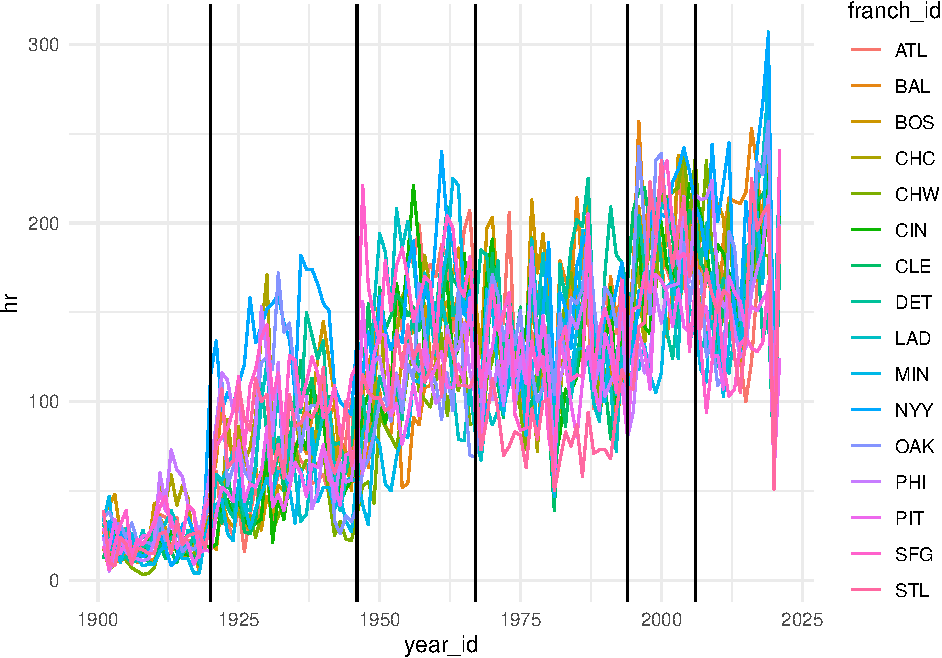
\includegraphics{paper_files/figure-latex/unnamed-chunk-1-1} \end{center}

\hypertarget{results-1}{%
\subsection{Results}\label{results-1}}

\begin{longtable}[]{@{}lrr@{}}
\toprule
franch\_id & threshold & years \\
\midrule
\endhead
NYY & 4.801818 & 1918 \\
BOS & 4.427752 & 1917 \\
BOS & 4.427752 & 1929 \\
BOS & 4.427752 & 1948 \\
BOS & 4.427752 & 1994 \\
LAD & 4.776867 & 1919 \\
LAD & 4.776867 & 1955 \\
ATL & 5.393778 & 1918 \\
ATL & 5.393778 & 1949 \\
CHW & 4.326192 & 1918 \\
CHC & 4.277577 & 1919 \\
CHC & 4.277577 & 1940 \\
CIN & 4.249476 & 1929 \\
CIN & 4.249476 & 1952 \\
CLE & 4.405339 & 1920 \\
CLE & 4.405339 & 1939 \\
DET & 3.926054 & 1927 \\
DET & 3.926054 & 1940 \\
BAL & 4.641706 & 1919 \\
BAL & 4.641706 & 1942 \\
SFG & 4.319634 & 1919 \\
SFG & 4.319634 & 1937 \\
OAK & 3.819294 & 1920 \\
OAK & 3.819294 & 1936 \\
OAK & 3.819294 & 1951 \\
PHI & 4.123104 & 1918 \\
PHI & 4.123104 & 1937 \\
PIT & 4.175793 & 1920 \\
PIT & 4.175793 & 1946 \\
STL & 5.444239 & 1919 \\
STL & 5.444239 & 1941 \\
MIN & 4.498666 & 1919 \\
MIN & 4.498666 & 1942 \\
\bottomrule
\end{longtable}

NYY 1918: Babe Ruth got to the Yankees in 1920. And starting in 1919
they had exactly one losing seasons between 1919 and 1965.\\
BOS 1917, 1929, 1948, 1994: Their last world series win in the 1900s was
in 1918.\\
I don't know 1929. 1948 there was a big jump in runs?\\
1994: Strike year.

LAD: 1919, 1955

ATL 1918 1949

CHW: 1919: Blaack Sox Scandal

CHC: 1919 1940 1940: War.

Cin: 1929 1952

CLE 1920 1939 Cleveland won the world series in 1920. Major change in
offensive output.

DET 1927 1940

BAL 1919 1942

SFG 1919 1937

OAK 1920 1936 1951

PHI 1918 1937

PIT 1920 1946

STL 1919 1941

MIN 1919 1942

Pearl Harbor was 1941. So US was in war in 1942.

\hypertarget{acknowledgements}{%
\section*{Acknowledgements}\label{acknowledgements}}
\addcontentsline{toc}{section}{Acknowledgements}

We thank Michael Lopez for suggesting we do ``something with change
point analysis.''

\hypertarget{supplementary-material}{%
\section*{Supplementary Material}\label{supplementary-material}}
\addcontentsline{toc}{section}{Supplementary Material}

All code for reproducing the analyses in this paper is publicly
available at \url{https://github.com/menawhalen/baseball_cpt}

\hypertarget{references}{%
\section*{References}\label{references}}
\addcontentsline{toc}{section}{References}

\hypertarget{refs}{}
\begin{CSLReferences}{1}{0}
\leavevmode\vadjust pre{\hypertarget{ref-Berry1999bridging}{}}%
Berry, Scott M., C. Shane Reese, and Patrick D. Larkey. 1999.
{``Bridging Different Eras in Sports.''} \emph{Journal of the American
Statistical Association} 94 (447): 661--76.
\url{https://doi.org/10.1080/01621459.1999.10474163}.

\leavevmode\vadjust pre{\hypertarget{ref-Cho2016}{}}%
Cho, H. 2016. {``Change-Point Detection in Panel Data via Double CUSUM
Statistic.''} \emph{Electronic Journal of Statistics} 10: 2000--2038.

\leavevmode\vadjust pre{\hypertarget{ref-hdbinseg}{}}%
Cho, Haeran, and Piotr Fryzlewicz. 2018. \emph{Hdbinseg: Change-Point
Analysis of High-Dimensional Time Series via Binary Segmentation}.
\url{https://CRAN.R-project.org/package=hdbinseg}.

\leavevmode\vadjust pre{\hypertarget{ref-ChoFryzlewwicz2014}{}}%
Cho, H., and P. Fryzlewicz. 2014. {``Multiple-Change-Point Detection for
High Dimensional Time Series via Sparsified Binary Segmentation.''}
\emph{JRSSB} 77: 475--507.

\leavevmode\vadjust pre{\hypertarget{ref-FortLee2007}{}}%
Fort R., Lee Y. H. 2007. {``Structural Change, Competitive Balance, and
the Rest of the Major Leagues.''} \emph{Economic Inquiry} 45 (3):
519--32.

\leavevmode\vadjust pre{\hypertarget{ref-Groothius2017}{}}%
Groothius, Peter A., Kurt W. Rotthoff, and Mark C. Strazicich. 2017.
{``Structural Breaks in the Game: The Case of Major League Baseball.''}
\emph{Journal of Sports Economics} 18 (6): 622--37.

\leavevmode\vadjust pre{\hypertarget{ref-LeeFort2005}{}}%
H., Lee Y., and Fort R. 2005. {``Structural Change in MLB Competitive
Balance: The Depression, Team Location, and Integration.''}
\emph{Economic Inquiry} 43 (1): 158--69.

\leavevmode\vadjust pre{\hypertarget{ref-PalaciosHuerta2004}{}}%
I., Palacios-Huerta. 2004. {``Structural Changes During a Century of the
World's Most Popular Sport.''} \emph{Statistical Methods and
Applications} 12: 241--58.

\leavevmode\vadjust pre{\hypertarget{ref-Nieswiadomy2012}{}}%
Nieswiadomy, Strazicich, M. L. 2012. {``Was There a Structural Break in
Barry Bonds's Bat?''} \emph{Journal of Quantitative Analysis in Sports}
8 (3).

\leavevmode\vadjust pre{\hypertarget{ref-BBHOF1869}{}}%
Rothenberg, Matt. n.d. \emph{PRO BASEBALL BEGAN IN CINCINNATI IN 1869}.
\url{https://baseballhall.org/discover/pro-baseball-began-in-cincinnati-in-1869\#:~:text=The\%20Cincinnati\%20Red\%20Stockings\%20made,professional\%20baseball\%20club\%20in\%201869.}

\leavevmode\vadjust pre{\hypertarget{ref-Woltring2018}{}}%
Woltring, Rost, M., and C. Jubenville. 2018. {``Examining Perceptions of
Baseball's Eras: A Statistical Comparison.''} \emph{The Sport Journal}.
\url{https://thesportjournal.org/article/examining-perceptions-of-baseballs-eras/}.

\end{CSLReferences}

\end{document}
